\documentclass{standalone}
\usepackage{tikz}
\usetikzlibrary{patterns, positioning}


\begin{document}
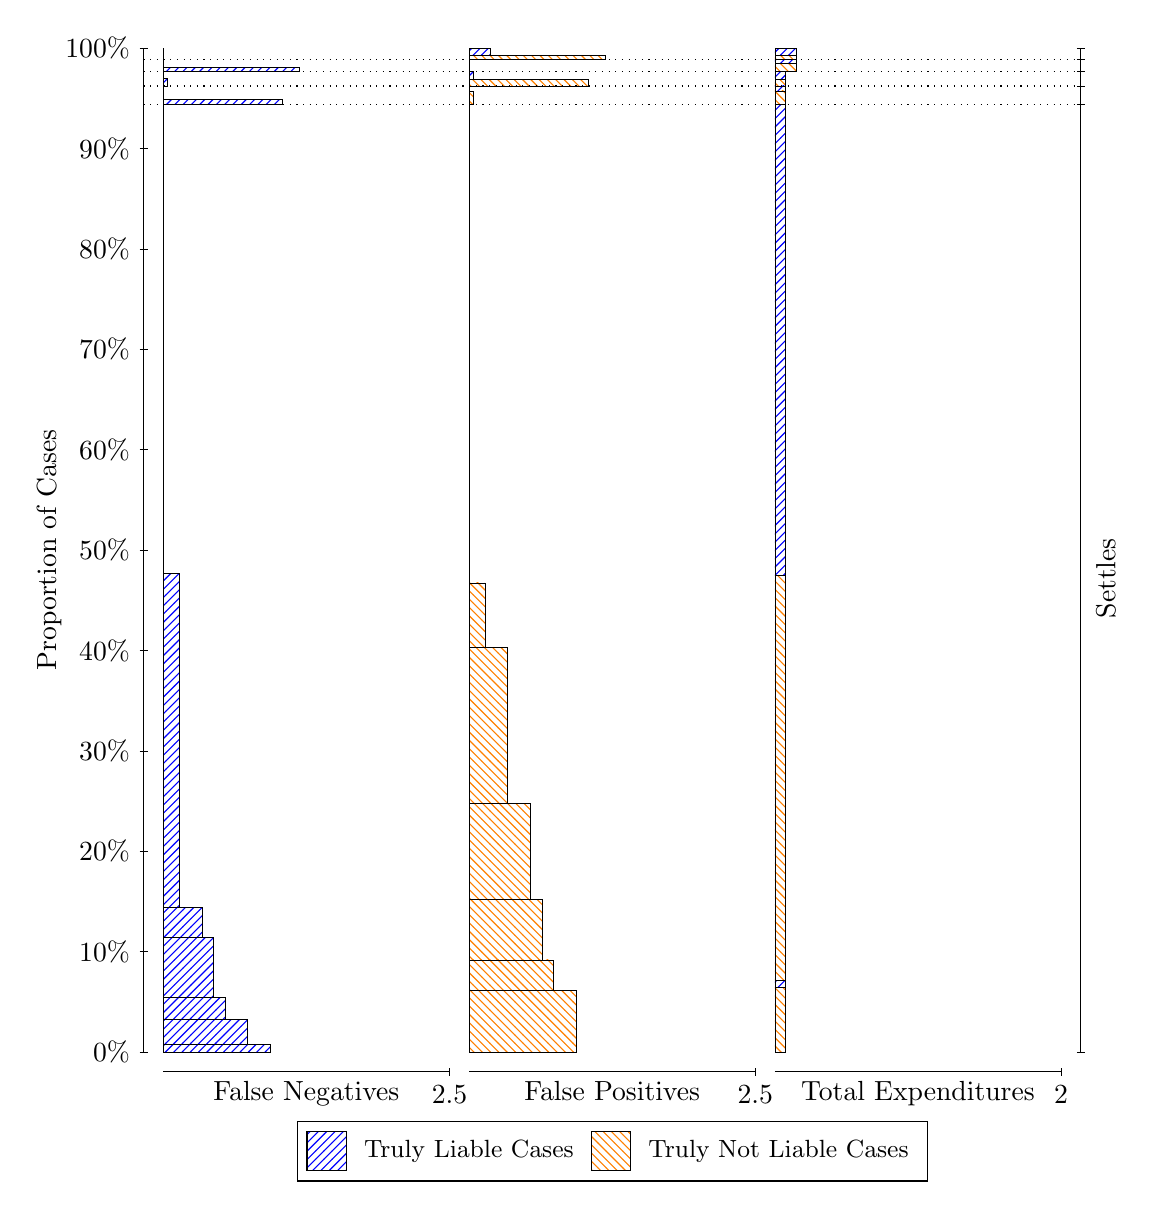
\begin{tikzpicture}
\draw[black, very thin] (1.5,1.75) -- (1.5,14.5);
\node[rotate=90, text=black, anchor=center] at (0.3, 8.125) {Proportion of Cases};
\draw[black, very thin] (1.45,1.75) -- (1.55,1.75);
\node[text=black, anchor=east] at (1.45, 1.75) {0\%};
\draw[black, very thin] (1.45,3.025) -- (1.55,3.025);
\node[text=black, anchor=east] at (1.45, 3.025) {10\%};
\draw[black, very thin] (1.45,4.3) -- (1.55,4.3);
\node[text=black, anchor=east] at (1.45, 4.3) {20\%};
\draw[black, very thin] (1.45,5.575) -- (1.55,5.575);
\node[text=black, anchor=east] at (1.45, 5.575) {30\%};
\draw[black, very thin] (1.45,6.85) -- (1.55,6.85);
\node[text=black, anchor=east] at (1.45, 6.85) {40\%};
\draw[black, very thin] (1.45,8.125) -- (1.55,8.125);
\node[text=black, anchor=east] at (1.45, 8.125) {50\%};
\draw[black, very thin] (1.45,9.4) -- (1.55,9.4);
\node[text=black, anchor=east] at (1.45, 9.4) {60\%};
\draw[black, very thin] (1.45,10.675) -- (1.55,10.675);
\node[text=black, anchor=east] at (1.45, 10.675) {70\%};
\draw[black, very thin] (1.45,11.95) -- (1.55,11.95);
\node[text=black, anchor=east] at (1.45, 11.95) {80\%};
\draw[black, very thin] (1.45,13.225) -- (1.55,13.225);
\node[text=black, anchor=east] at (1.45, 13.225) {90\%};
\draw[black, very thin] (1.45,14.5) -- (1.55,14.5);
\node[text=black, anchor=east] at (1.45, 14.5) {100\%};

\draw[black, very thin] (13.4,1.75) -- (13.4,14.5);
\draw[black, very thin] (13.35,1.75) -- (13.45,1.75);
\node[anchor=west] at (13.35, 1.75) {};
\draw[black, very thin] (13.35,13.781) -- (13.45,13.781);
\node[anchor=west] at (13.35, 13.781) {};
\draw[black, very thin] (13.35,14.018) -- (13.45,14.018);
\node[anchor=west] at (13.35, 14.018) {};
\draw[black, very thin] (13.35,14.199) -- (13.45,14.199);
\node[anchor=west] at (13.35, 14.199) {};
\draw[black, very thin] (13.35,14.359) -- (13.45,14.359);
\node[anchor=west] at (13.35, 14.359) {};
\draw[black, very thin] (13.35,14.5) -- (13.45,14.5);
\node[anchor=west] at (13.35, 14.5) {};

\draw[black, very thin, pattern color=blue, pattern=north east lines] (1.75,1.75) rectangle (3.1125,1.8472);
\draw[black, very thin, pattern color=blue, pattern=north east lines] (1.75,1.8472) rectangle (2.8218,2.164);
\draw[black, very thin, pattern color=blue, pattern=north east lines] (1.75,2.164) rectangle (2.5312,2.4442);
\draw[black, very thin, pattern color=blue, pattern=north east lines] (1.75,2.4442) rectangle (2.3858,3.2076);
\draw[black, very thin, pattern color=blue, pattern=north east lines] (1.75,3.2076) rectangle (2.2405,3.591);
\draw[black, very thin, pattern color=blue, pattern=north east lines] (1.75,3.591) rectangle (1.9498,7.8232);
\draw[black, very thin, pattern color=orange, pattern=north west lines] (1.75,7.8232) rectangle (1.75,13.781);
\draw[black, very thin, pattern color=blue, pattern=north east lines] (1.75,13.781) rectangle (3.2578,13.843);
\draw[black, very thin, pattern color=orange, pattern=north west lines] (1.75,13.843) rectangle (1.75,14.018);
\draw[black, very thin, pattern color=blue, pattern=north east lines] (1.75,14.018) rectangle (1.8045,14.117);
\draw[black, very thin, pattern color=orange, pattern=north west lines] (1.75,14.117) rectangle (1.75,14.199);
\draw[black, very thin, pattern color=blue, pattern=north east lines] (1.75,14.199) rectangle (3.4758,14.252);
\draw[black, very thin, pattern color=orange, pattern=north west lines] (1.75,14.252) rectangle (1.75,14.359);
\draw[black, very thin, pattern color=orange, pattern=north west lines] (1.75,14.359) rectangle (1.75,14.411);
\draw[black, very thin, pattern color=blue, pattern=north east lines] (1.75,14.411) rectangle (1.75,14.5);
\draw[black, very thin, pattern color=orange, pattern=north west lines] (5.6333,1.75) rectangle (6.9958,2.5352);
\draw[black, very thin, pattern color=orange, pattern=north west lines] (5.6333,2.5352) rectangle (6.7052,2.9187);
\draw[black, very thin, pattern color=orange, pattern=north west lines] (5.6333,2.9187) rectangle (6.5598,3.6836);
\draw[black, very thin, pattern color=orange, pattern=north west lines] (5.6333,3.6836) rectangle (6.4145,4.9108);
\draw[black, very thin, pattern color=orange, pattern=north west lines] (5.6333,4.9108) rectangle (6.1238,6.8918);
\draw[black, very thin, pattern color=orange, pattern=north west lines] (5.6333,6.8918) rectangle (5.8332,7.7077);
\draw[black, very thin, pattern color=blue, pattern=north east lines] (5.6333,7.7077) rectangle (5.6333,13.781);
\draw[black, very thin, pattern color=orange, pattern=north west lines] (5.6333,13.781) rectangle (5.6878,13.957);
\draw[black, very thin, pattern color=blue, pattern=north east lines] (5.6333,13.957) rectangle (5.6333,14.018);
\draw[black, very thin, pattern color=orange, pattern=north west lines] (5.6333,14.018) rectangle (7.1412,14.1);
\draw[black, very thin, pattern color=blue, pattern=north east lines] (5.6333,14.1) rectangle (5.6878,14.199);
\draw[black, very thin, pattern color=orange, pattern=north west lines] (5.6333,14.199) rectangle (5.6333,14.307);
\draw[black, very thin, pattern color=blue, pattern=north east lines] (5.6333,14.307) rectangle (5.6333,14.359);
\draw[black, very thin, pattern color=orange, pattern=north west lines] (5.6333,14.359) rectangle (7.3592,14.411);
\draw[black, very thin, pattern color=blue, pattern=north east lines] (5.6333,14.411) rectangle (5.9058,14.5);
\draw[black, very thin, pattern color=orange, pattern=north west lines] (9.5167,1.75) rectangle (9.6529,2.566);
\draw[black, very thin, pattern color=blue, pattern=north east lines] (9.5167,2.566) rectangle (9.6529,2.6631);
\draw[black, very thin, pattern color=orange, pattern=north west lines] (9.5167,2.6631) rectangle (9.6529,7.8049);
\draw[black, very thin, pattern color=blue, pattern=north east lines] (9.5167,7.8049) rectangle (9.6529,13.781);
\draw[black, very thin, pattern color=orange, pattern=north west lines] (9.5167,13.781) rectangle (9.6529,13.957);
\draw[black, very thin, pattern color=blue, pattern=north east lines] (9.5167,13.957) rectangle (9.6529,14.018);
\draw[black, very thin, pattern color=orange, pattern=north west lines] (9.5167,14.018) rectangle (9.6529,14.1);
\draw[black, very thin, pattern color=blue, pattern=north east lines] (9.5167,14.1) rectangle (9.6529,14.199);
\draw[black, very thin, pattern color=orange, pattern=north west lines] (9.5167,14.199) rectangle (9.7892,14.307);
\draw[black, very thin, pattern color=blue, pattern=north east lines] (9.5167,14.307) rectangle (9.7892,14.359);
\draw[black, very thin, pattern color=orange, pattern=north west lines] (9.5167,14.359) rectangle (9.7892,14.411);
\draw[black, very thin, pattern color=blue, pattern=north east lines] (9.5167,14.411) rectangle (9.7892,14.5);
\draw[black, dotted] (1.5,13.781) -- (13.4,13.781);
\draw[black, dotted] (1.5,14.018) -- (13.4,14.018);
\draw[black, dotted] (1.5,14.199) -- (13.4,14.199);
\draw[black, dotted] (1.5,14.359) -- (13.4,14.359);
\draw[black, very thin] (1.75,1.5) -- (5.3833,1.5);
\node[text=black, anchor=north] at (3.5667, 1.5) {False Negatives};
\draw[black, very thin] (5.3833,1.45) -- (5.3833,1.55);
\node[text=black, anchor=north] at (5.3833, 1.45) {2.5};

\draw[black, very thin] (5.6333,1.5) -- (9.2667,1.5);
\node[text=black, anchor=north] at (7.45, 1.5) {False Positives};
\draw[black, very thin] (9.2667,1.45) -- (9.2667,1.55);
\node[text=black, anchor=north] at (9.2667, 1.45) {2.5};

\draw[black, very thin] (9.5167,1.5) -- (13.15,1.5);
\node[text=black, anchor=north] at (11.333, 1.5) {Total Expenditures};
\draw[black, very thin] (13.15,1.45) -- (13.15,1.55);
\node[text=black, anchor=north] at (13.15, 1.45) {2};

\node[text=black, centered, rotate=90] at (13.72, 7.7655) {Settles};





\draw (7.449999999999999,1.5) node[draw=none] (baseCoordinate) {};
\begin{scope}[align=center]
        \matrix[scale=0.5, draw=black, below=0.5cm of baseCoordinate, nodes={draw}, column sep=0.1cm]{
            \node[rectangle, draw, minimum width=0.5cm, minimum height=0.5cm, pattern color=blue, pattern=north east lines] {}; &
            \node[draw=none, font=\small, text=black] (B) {Truly Liable Cases}; &
            \node[rectangle, draw, minimum width=0.5cm, minimum height=0.5cm, pattern color=orange, pattern=north west lines] {}; &
            \node[draw=none, font=\small, text=black] (B) {Truly Not Liable Cases}; \\
            };
\end{scope}

\end{tikzpicture}
\end{document}